\documentclass[11pt]{article}
\usepackage{amsmath, amssymb, amscd, amsthm, amsfonts}
\usepackage{graphicx}
\usepackage{hyperref}
\usepackage{subfigure}
\usepackage{float}
\usepackage{rotating}
\usepackage{tikz}
\usepackage{xcolor}
\usepackage{listings}
\definecolor{vgreen}{RGB}{104,180,104}
\definecolor{vblue}{RGB}{49,49,255}
\definecolor{vorange}{RGB}{255,143,102}
\lstdefinestyle{verilog-style}
{
    language=Verilog,
    basicstyle=\small\ttfamily,
    keywordstyle=\color{vblue},
    identifierstyle=\color{black},
    commentstyle=\color{vgreen},
    numbers=left,
    numberstyle=\tiny\color{black},
    numbersep=10pt,
    tabsize=4,
    moredelim=*[s][\colorIndex]{[}{]},
    literate=*{:}{:}1
}

\makeatletter
\newcommand*\@lbracket{[}
\newcommand*\@rbracket{]}
\newcommand*\@colon{:}
\newcommand*\colorIndex{%
    \edef\@temp{\the\lst@token}%
    \ifx\@temp\@lbracket \color{black}%
    \else\ifx\@temp\@rbracket \color{black}%
    \else\ifx\@temp\@colon \color{black}%
    \else \color{vorange}%
    \fi\fi\fi
}
\makeatother

\usepackage{trace}



\oddsidemargin 0pt
\evensidemargin 0pt
\marginparwidth 40pt
\marginparsep 10pt
\topmargin -20pt
\headsep 10pt
\textheight 8.7in
\textwidth 6.65in
\linespread{1.2}

\title{Digital Bubble Level - Cadence RTL Synthesis}
\author{Vladislav Pomogaev - 26951160}
\date{October 10, 2021}

\newcommand{\rr}{\mathbb{R}}

\newcommand{\al}{\alpha}
\DeclareMathOperator{\conv}{conv}
\DeclareMathOperator{\aff}{aff}

\begin{document}

\maketitle

\section{Introduction}
In this assignment, the original bubble level FSM was synthesised in Cadence using elements from the FreePDK15 library. The compiled Verilog module was transformed into logic gates/elements from the library with simulated delays. I note a presence of delays proportional to the delay of elements in the data paths. 170 cells are in the final design.

To make use of the functional simulation, the clock parameters were adjusted to match the worst-case real-world scenario. The clock timing constraint was set to 200MHz; simulation speed to 100MHz, and the execution target frequency on the FPGA is 50MHz. I do this to give the design lots of clock headroom in case someone want overclock by x2 (Note that the I\textsuperscript{2}C controller has an operating frequency of either 100MHz or 50MHz). 

\section{Outputs of RTL Compiler}

\begin{figure}[H]
    \centering
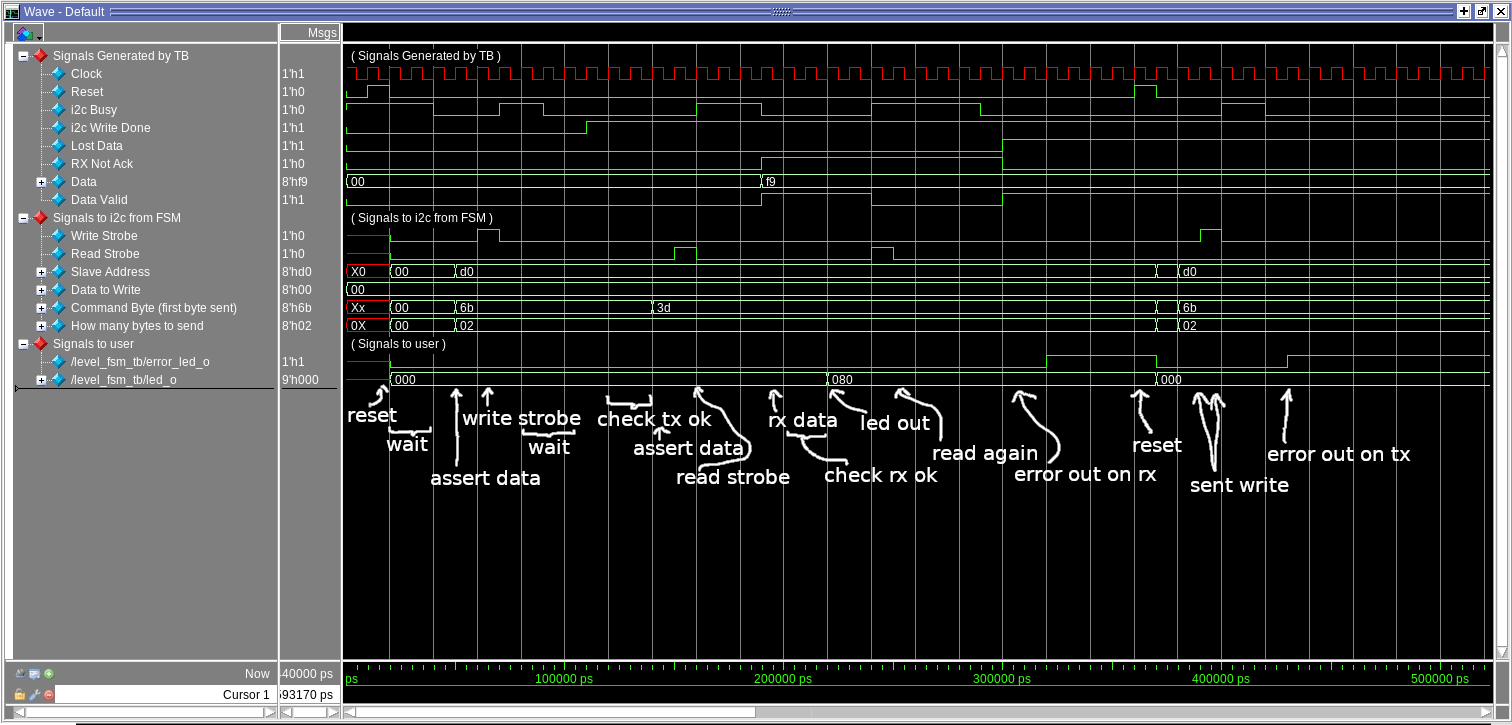
\includegraphics[width=0.99\textwidth]{delayed_wave2.png}
    \caption{The original test bench was run on the newly compiled design. The test bench passed all assertions as last time due to the fact that all assertions were on the next clock cycle after a state change. The simulation frequency was adjusted from 1GHz to 100MHz to reflect the more accurate timing when run at 50MHz on the FPGA. The clock constraint was also adjusted to 200MHz to ensure positive slack and lots of headroom. }
\end{figure}
\begin{figure}[H]
    \centering
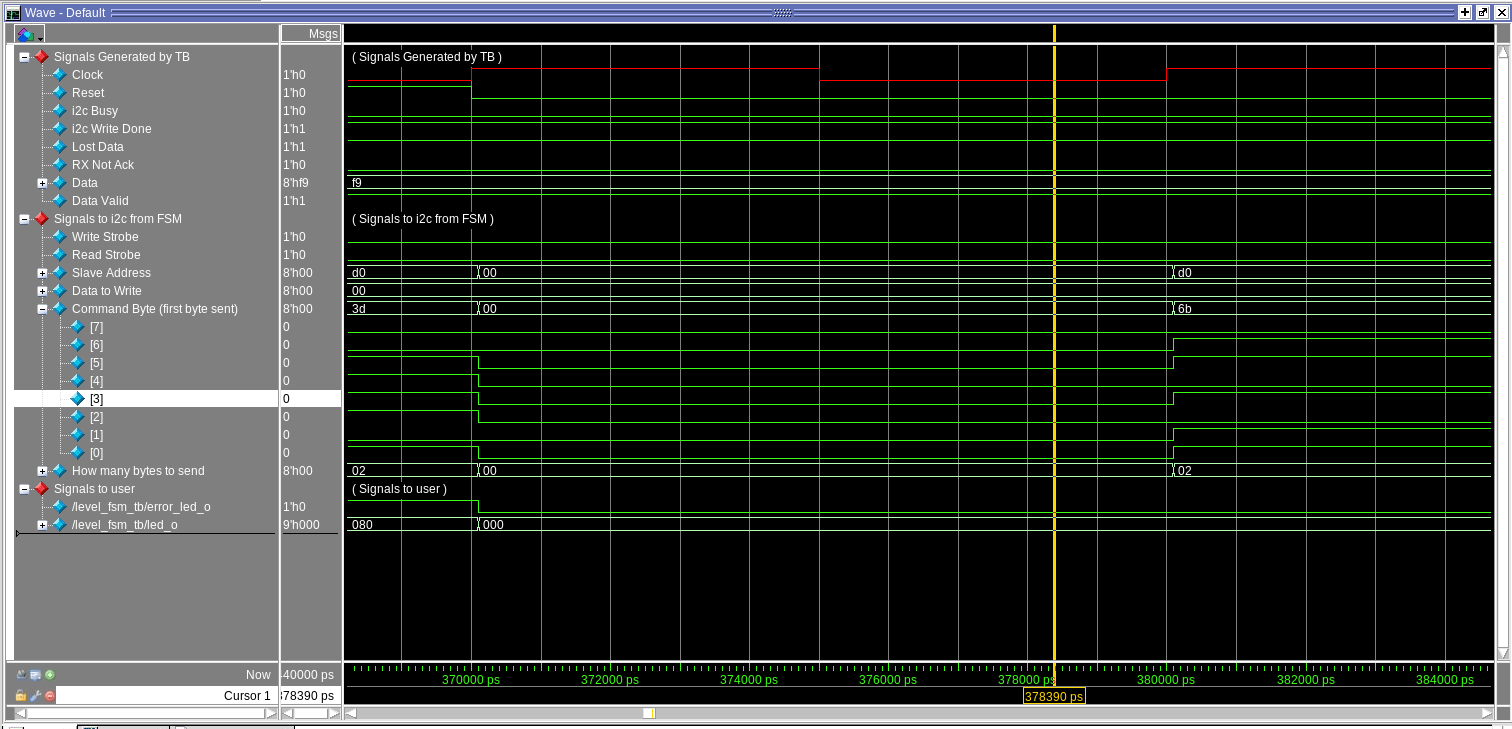
\includegraphics[width=0.99\textwidth]{closeup_delayed_wave.png}
    \caption{We see some changes from the previous simulation. Most notably, there is now delay between the clock and the output of signals from the FSM. These delays are different for different signals as expected. There are still no delays in the input of signals though because that was part of the original test bench. We make the assumption that the signals arrive at or before clock change. In this figure at around 380000ps we see the delay of the command byte relative to the reference clock. I assume if our signal was to propagate at uneven times through a combinational circuit we would see that in this simulation. However, all signals are from registers, so we cannot see a difference in the arrival of different signals on the same bus. Since the frequency we are running this project at is so low compared to the actual frequency, the delays have little effect on the functionality of the circuit.}
\end{figure}

I note here that the following synthesis parameters effect the simulation in the following ways:
\begin{itemize}
  \item timing.sdc file has a clock constraint that Cadence RTL designer uses to verify and optimize layout for set-up, slack and hold times. Increasing the clock frequency makes the compiler work harder (more optimization) to align the cells in a way to meet the constraints. 
  \item test bench timescale sets the scale for delays in the simulation, and the resolution at which the simulation is done.
\end{itemize}

\section{Outputs of RTL Compiler}
\subsection{Reports}
level{\_}fsm{\_}area.rpt
\lstinputlisting[style={}, basicstyle=\tiny,]{synth/out/level_fsm_area.rpt}
level{\_}fsm{\_}gates.rpt
\lstinputlisting[style={}, basicstyle=\tiny,]{synth/out/level_fsm_gates.rpt}
level{\_}fsm{\_}power.rpt
\lstinputlisting[style={}, basicstyle=\tiny,]{synth/out/level_fsm_power.rpt}
level{\_}fsm{\_}timing.rpt
\lstinputlisting[style={}, basicstyle=\tiny,]{synth/out/level_fsm_timing.rpt}
\subsection{Mapped Verilog}
level{\_}fsm{\_}map.v
\lstinputlisting[style={verilog-style}, basicstyle=\tiny,]{synth/out/level_fsm_map.v}

\end{document}